
un automa a stati finiti ha un insieme di stati e un controllo che si muove da stato a stato in risposta a input esterni. Si ha una distinzione:
\begin{itemize}
\item \textbf{automi deterministici:} dove l'automa non può essere in più di uno stato per volta
\item \textbf{automi non deterministici:} dove l'automa può trovarsi in più stati contemporaneamente
\end{itemize}
\subsection{Automi deterministici}
Un automa a stati finiti deterministico (\textit{DFA}), un automa che dopo aver letto una qualunque sequenza di input si trova in un singolo stato. Il termine \textit{deterministico} concerne il fatto che per ogni input esiste un solo stato verso il quale l'automa passa dal suo stato corrente. Un automa a stati finiti deterministico consiste nelle seguenti parti:
\begin{itemize}
\item un insieme finito di stati, spesso indicato con $Q$
\item un insieme finito di simboli di input , spesso indicato con $\Sigma$
\item una funzione di transizione, che prende come argomento uno stato e un simbolo di input e restituisce uno stato. La funzione di transizione sarà indicata comunemente con $\delta$. Nella rappresentazione grafica informale di automi $\delta$ è rappresentata dagli archi tra gli stati e dalle etichette sugli archi. Se $q$ è uno stato e $a$ è un simbolo di input, $\delta(q,a)$ è lo stato $p$ tale che esiste un arco etichettato con $a$ da $q$ a $p^2$
\item uno stato iniziale, uno degli stati in $Q$
\item un insieme di stati finali, o accettanti , $F$. L'insieme $F$ è un sottoinsieme di $Q$
\end{itemize}
Nel complesso un DFA è rappresentato in maniera concisa con l'enumerazione dei suoi elementi, quindi con la quintupla:
$$A=(Q,\Sigma,\delta,q_0,F)$$
con $A$ nome del DFA, $Q$ insiem degli stati, $\Sigma$ rappresentante i simboli di input, $\delta$ la sua funzione di transizione, $q_0$ il suo stato iniziale e $F$ l'insieme degli stati accettanti.\\
Vediamo come decidere se accettare o meno una stringa (sequenza di caratteri) in input mediante un DFA.\\
Ho una sequenza in input $a_1...a_n$. Parto dallo stato iniziale $q_0$, consultando la funzione di transizione $\delta$, per esempio  $\delta(q_0,a_1)=q_1$ e trovo lo stato in cui il DFA entra dopo aver letto $a_1$. Poi passo a $\delta(q_1,a_2)=q_2$ e così via, $\delta(q_{i-1},a_i)=q_i$ fino a ottenere $q_n$. Se $q_n$ è elemento di $F$ allora $a_1...a_n$ viene accettato, altrimenti viene rifiutato.
\begin{esempio}
specifico DFA che accetta tutte le strighe binarie in cui compare la sequenza 01:
$$L=\{w|w \mbox{ è della forma x01y, con x e y pari a 0 o 1} \}=\{01,11010,100011,...\}$$
o anche:
$$L=\{x01y| x,y\in\{0,1\}^* \}$$
abbiamo quindi:
$$\Sigma=\{0,1\}$$
ragioniamo sul fatto che $A$:
\begin{enumerate}
\item se ha "già visto" 01, accetterà qualsiasi input
\item pur non avendo ancora visto 01, l'input più recente è stato 0, cosicché se ora vede un 1 avrà visto 01
\item non ha ancora visto 01, ma l'input più recente è nullo (siamo all'inizio), in tal caso A non accetta finché non vede
uno 0 e subito dopo un 1
\end{enumerate} 
la terza condizione rappresenta lo stato iniziale. All'inizio bisogna vedere uno 0 e poi un 1. Ma se nello stato $q_0$ si vede per primo un 1 allora non abbiamo fatto alcun passo verso 01, e dunque dobbiamo permanere nello stato $q_0$, $\delta(q_0,1)=q_0$. D'altra parte se nello stato iniziale vedo 0 siamo nella seconda condizione, uso quindi $q_2$ per questa condizione, si avrà quindi $\delta(q_0,0)=q_2$. Vedo ora le transizoni di $q_2$, se vedo 0 ho che 0 è l'ultimo simbolo incontrato quindi uso nuovamente $q_2$, $\delta(q_2,0)=q_2$, in attesa di un 1. Se arriva 1 passo allo stato accertante $q_1$ corrispondente alla prima condizione, $\delta(q_2,1)=q_1$. Ora abbiamo incontrato 01 quindi può succedere qualsiasi cosa e dopo qualsiasi cosa accada potremo nuovamente aspettarci qualsiasi cosa, ovvero $\delta(q_1,0)=\delta(q_1,1)=q_1$. Si deduce quindi che:
$$Q=\{q_0,q_1,q_2\} \mbox{ e } F=\{q_1\}$$
quindi:
$$A=\{\{q_0,q_1,q_2\} ,\{0,1\}, \delta, q_0, \{q_1\} \}$$
con in totale le seguenti transizioni:
$$\delta(q_0,1)=q_0$$
$$\delta(q_0,0)=q_2$$
$$\delta(q_2,0)=q_2$$
$$\delta(q_2,1)=q_1$$
$$\delta(q_1,0)=q_1$$
$$\delta(q_1,1)=q_1$$
posso rappresentarle in maniera tabulare, con lo stato inizale indicato da $\to$ e quelli accettanti con $*$:
\begin{center}
\begin{tabular}{c|c|c}
$\delta$ & 0 & 1 \\
\hline
$\to\,q_0$ & $q_1$ & $q_0$\\
\hline
$*\,q_1$ & $q_1$ & $q_1$\\
\hline
$q_2$ & $q_2$ & $q_1$
\end{tabular}
\end{center}
o col diagramma di transizione:
\begin{center}
\begin{tikzpicture}[shorten >=1pt,node distance=2cm,on grid,auto] 
   \node[state,initial] (q_0)   {$q_0$}; 
   \node[state] (q_2) [right=of q_0] {$q_2$}; 
   \node[state, accepting] (q_1) [right=of q_2] {$q_1$}; 
   \path[->] 
   (q_0) edge  node {0} (q_2)
         edge [loop below] node {1} ()
   (q_2) edge  node  {1} (q_1)
         edge [loop below] node {0} ()
   (q_1) edge [loop below] node {0,1} ();
\end{tikzpicture}

\end{center}
\end{esempio}
\newpage
\begin{esempio}
Trovo automa per: $$L=\{w\in\{a,b\}^*|\mbox{ w che contiene un numero pari di b}\}$$
\begin{center}
\begin{tikzpicture}[shorten >=1pt,node distance=3cm,on grid,auto] 
	\node[state, initial, accepting] (q_0) {$q_0$};
	\node[state] (q_1) [right=of q_0] {$q_1$};
	\path[->]
	(q_0) edge [bend left = 25] node {b} (q_1)
	      edge [loop below] node {a} ()
	(q_1) edge [bend left = 25] node {b} (q_0)
	      edge [loop below] node {a} ();
\end{tikzpicture}
\end{center}
ovvero se da $q_0$ vado a $q_1$ sono obbligato ab generare due $b$, dato che il nodo accettnate è $q_0$. In entrambi i nodi posso generare quante $a$ voglio.
\end{esempio}
\begin{esempio}
Trovo automa per: $$L=\{w\in\{a,b\}^*|\mbox{ w che contiene un numero dispari di b}\}$$
\begin{center}
\begin{tikzpicture}[shorten >=1pt,node distance=3cm,on grid,auto] 
	\node[state, initial] (q_0) {$q_0$};
	\node[state, accepting] (q_1) [right=of q_0] {$q_1$};
	\path[->]
	(q_0) edge [bend left = 25] node {b} (q_1)
	      edge [loop below] node {a} ()
	(q_1) edge [bend left = 25] node {b} (q_0)
	      edge [loop below] node {a} ();
\end{tikzpicture}
\end{center}
ovvero se da $q_0$ vado a $q_1$ sono obbligato ab generare una sola $b$, dato che il nodo accettnate è $q_1$. In entrambi i nodi posso generare quante $a$ voglio e posso tornare da $q_1$ a $q_0$ per generare altre $b$.
\end{esempio}
\begin{esempio}
Trovo automa per: $$L=\{w\in\{0,1\}^*| w= 0^n1^m\}$$
vediamo i vari casi:
\textbf{Si ha che} $q_E$ \textbf{è lo stato pozzo dove vanno le stringhe venute male}
\begin{itemize}
\item $n,m\geq 0$:
\begin{center}
\begin{tikzpicture}[shorten >=1pt,node distance=2cm,on grid,auto] 
   \node[state,initial, accepting] (q_0)   {$q_0$}; 
   \node[state, accepting] (q_1) [right=of q_0] {$q_1$}; 
   \node[state] (q_E) [right=of q_1] {$q_E$}; 
   \path[->] 
   (q_0) edge  node {1} (q_1)
         edge [loop below] node {0} ()
   (q_1) edge  node  {} (q_E)
         edge [loop below] node {1} ()
   (q_E) edge [loop below] node {0,1} ();
\end{tikzpicture}
\end{center}
ovvero posso non generare nulla e uscire subito con $q_0$, generare solo un 1 e passare a $q_1$ e uscire oppure generare 0 e 1 a piacere con l'ultimo stato o generare 0 a piacere dal primo e 1 a piacere dal secondo.
\item $n\geq 0 \,\,m>0$:
\begin{center}
\begin{tikzpicture}[shorten >=1pt,node distance=2cm,on grid,auto] 
   \node[state,initial] (q_0)   {$q_0$}; 
   \node[state, accepting] (q_1) [right=of q_0] {$q_1$}; 
   \node[state] (q_E) [right=of q_1] {$q_E$}; 
   \path[->] 
   (q_0) edge  node {1} (q_1)
         edge [loop below] node {0} ()
   (q_1) edge  node  {} (q_E)
         edge [loop below] node {1} ()
   (q_E) edge [loop below] node {0,1} ();
\end{tikzpicture}
\end{center}
ovvero come l'esempio sopra solo che non posso uscire in $q_0$ in quanto almeno un 1 deve essere per forza generato
\item $n> 0\,\, m\geq 0$:
\begin{center}
\begin{tikzpicture}[shorten >=1pt,node distance=2cm,on grid,auto] 
   \node[state,initial] (q_0)   {$q_0$}; 
   \node[state, accepting] (q_1) [right=of q_0] {$q_1$}; 
   \node[state, accepting] (q_2) [right=of q_1] {$q_2$}; 
   \node[state] (q_E) [right=of q_2] {$q_E$}; 
   \path[->] 
   (q_0) edge  node {0} (q_1)
         edge [bend right] node {1} (q_E)
   (q_1) edge  node {1} (q_2)
         edge [loop above] node {0} ()
   (q_2) edge node {0} (q_E)
         edge [loop above] node {1} ()
   (q_E) edge [loop below] node {0,1} ();
\end{tikzpicture}
\end{center}
\textit{CHIARIRE}
\item $n,m>0$:
\begin{center}
\begin{tikzpicture}[shorten >=1pt,node distance=2cm,on grid,auto] 
   \node[state,initial] (q_0)   {$q_0$}; 
   \node[state] (q_1) [right=of q_0] {$q_1$}; 
   \node[state, accepting] (q_2) [right=of q_1] {$q_2$}; 
   \node[state] (q_E) [right=of q_2] {$q_E$}; 
   \path[->] 
   (q_0) edge  node {0} (q_1)
         edge [bend right] node {1} (q_E)
   (q_1) edge  node {1} (q_2)
         edge [loop above] node {0} ()
   (q_2) edge node {0} (q_E)
         edge [loop above] node {1} ()
   (q_E) edge [loop below] node {0,1} ();
\end{tikzpicture}
\end{center}
\textit{CHIARIRE}
\end{itemize}
\end{esempio}
\newpage
\begin{esempio}
Trovo automa per: $$L=\{w\in\{a,b\}^*|\mbox{ w che contiene un numero pari di a e dispari di b}\}$$
\begin{center}
\begin{tikzpicture}[shorten >=1pt,node distance=2cm,on grid,auto] 
	\node[state, initial] (q_0) {$q_{pp}$};
	\node[state] (q_1) [right=of q_0] {$q_{dp}$};
	\node[state, accepting] (q_2) [below=of q_0] {$q_{pd}$};
	\node[state] (q_3) [right=of q_2] {$q_{dd}$};
	\path[->]
	(q_0) edge [bend left = 25] node {a} (q_1)
	      edge [bend right = 25] node [left] {b} (q_2)
	(q_1) edge [bend left = 25] node {a} (q_0)
	      edge [bend right = 25] node [left] {b} (q_3)
	(q_2) edge [bend right = 25] node [right] {b} (q_0)
	      edge [bend left = 25] node {a} (q_3)
	(q_3) edge [bend right = 25] node [right] {b} (q_1)
	      edge [bend left = 25] node {a} (q_2);
\end{tikzpicture}
\end{center}
\end{esempio}
\begin{esempio}
Trovo automa per: $$L=\{w\in\{a,b\}^*|\mbox{ w che contiene un numero pari di a seguito da uno dispari di b}\}$$
$$L=\{a^{2n}b^{2k+1}|j,k\geq 0\}$$
\begin{center}
\begin{tikzpicture}[shorten >=1pt,node distance=2cm,on grid,auto] 
	\node[state, initial] (q_0) {$q_{0}$};
	\node[state, accepting] (q_1) [right=of q_0] {$q_{1}$};
	\node[state] (q_2) [below=of q_0] {$q_{2}$};
	\node[state] (q_3) [right=of q_2] {$q_3$};
	\node[state] (q_4) [right = of q_3] {$q_E$};
	\path[->]
	(q_0) edge [bend left = 25] node {b} (q_1)
	      edge [bend right = 25] node [left] {a} (q_2)
	(q_1) edge [bend left = 25] node {a} (q_4)
	      edge [bend right = 25] node [left] {b} (q_3)
	(q_2) edge [bend right = 25] node [below] {b} (q_4)
	      edge [bend right = 25] node [right] {a} (q_0)
	(q_3) edge [bend right = 25] node [right] {b} (q_1)
	      edge [bend left = 25] node {a} (q_4);
\end{tikzpicture}
\end{center}
ovvero in tabella:
\begin{center}
\begin{tabular}{c|c|c}
$\delta$ & a & b \\
\hline
$\to\,q_0$ & $q_1$ & $q_2$\\
\hline
$q_1$ & $q_0$ & $q_E$\\
\hline
$*\,q_2$ & $q_E$ & $q_3$\\
\hline
$q_3$ & $q_E$ & $q_2$\\
\hline
$q_E$ & $q_E$ & $q_E$
\end{tabular}
\end{center}
\end{esempio}
\begin{esempio}
Trovo automa per: $$L=\{a^{2k+1}b^{2h}|\, h,k\geq 0\}$$
\begin{center}
\begin{tikzpicture}[shorten >=1pt,node distance=2cm,on grid,auto] 
	\node[state, initial] (q_0) {$q_{0}$};
	\node[state, accepting] (q_1) [right=of q_0] {$q_{1}$};
	\node[state] (q_3) [right=of q_1] {$q_{3}$};
	\node[state] (q_2) [below= of q_1] {$q_{2}$};
	\node[state, accepting] (q_4) [right = of q_2] {$q_4$};
	\node[state] (q_5) [right=of q_4] {$q_E$};
	\path[->]
	(q_0) edge  node [bend left = 25] {a} (q_1)
	(q_1) edge [bend left = 25] node {a} (q_2)
	      edge node [bend left= 25] {b} (q_3)
	(q_2) edge [bend left = 25] node [left] {a} (q_1)
	(q_3) edge [bend right = 25] node [left] {b} (q_4)
	(q_4) edge [bend right = 25] node {} (q_3);
\end{tikzpicture}
\end{center}
\end{esempio}
\begin{esempio}
Trovo automa per: $$L=\{a^{2n+1}b^{2k+1}|\, n,k\geq 0\}$$
\begin{center}
\begin{tikzpicture}[shorten >=1pt,node distance=2cm,on grid,auto] 
	\node[state, initial] (q_0) {$q_{0}$};
	\node[state] (q_1) [right=of q_0] {$q_{1}$};
	\node[state, accepting] (q_3) [right=of q_1] {$q_{3}$};
	\node[state] (q_2) [below= of q_1] {$q_{2}$};
	\node[state] (q_4) [right = of q_2] {$q_4$};
	\node[state] (q_5) [right=of q_4] {$q_E$};
	\path[->]
	(q_0) edge  node [bend left = 25] {a} (q_1)
	(q_1) edge [bend left = 25] node {a} (q_2)
	      edge node [bend left= 25] {b} (q_3)
	(q_2) edge [bend left = 25] node [left] {a} (q_1)
	(q_3) edge [bend right = 25] node [left] {b} (q_4)
	(q_4) edge [bend right = 25] node [right] {b} (q_3);
\end{tikzpicture}
\end{center}
\end{esempio}
\begin{esempio}
Trovo automa per: $$L=\{x010y|\,x,y\in\{o,1\}^*\}$$
\begin{center}
\begin{tikzpicture}[shorten >=1pt,node distance=2cm,on grid,auto] 
	\node[state, initial] (q_0) {$q_{0}$};
	\node[state] (q_1) [right=of q_0] {$q_{1}$};
	\node[state] (q_2) [right=of q_1] {$q_{2}$};
	\node[state, accepting] (q_3) [right= of q_2] {$q_{3}$};
	\path[->]
	(q_0) edge  node {0} (q_1)
	      edge [loop above] node {1} ()
	(q_1) edge  node {1} (q_2)
	      edge [loop above] node {0} ()
	(q_2) edge  node {0} (q_3)
	(q_3) edge [loop below] node {0,1} ();
\end{tikzpicture}
\end{center}
\end{esempio}
\subsection{Automi non deterministici}
Un automa a stati finiti non deterministici (\textit{NFA}) può trovarsi in diversi stati contemporaneamente. Come i DFA accettano linguaggi regolari e spesso sono più semplici da trattare rispetto ai DFA.\\
Un NFA è definito come un NFA ma si ha un diverso tipo di transizione $\delta$, che ha sempre come argomenti uno stato e un simbolo di input ma resituisce zero o più stati.
\begin{esempio}
Sia $L=\{x01|\,x\in\{o,1\}$ ovvero il linguaggio formato da tutte le stringhe binarie che terminano in 01.\\
Avremo il seguente automa determinsitico:
\begin{center}
\begin{tikzpicture}[shorten >=1pt,node distance=2cm,on grid,auto] 
	\node[state, initial] (q_0) {$q_{0}$};
	\node[state] (q_1) [right=of q_0] {$q_{1}$};
	\node[state, accepting] (q_2) [right=of q_1] {$q_{2}$};
	\path[->]
	(q_0) edge  node {0} (q_1)
	      edge [loop above] node {1} ()
	(q_1) edge  node {1} (q_2)
	      edge [loop above] node {0} ()
	(q_2) edge  [bend left =25] node {0} (q_1)
	      edge [bend left = 50] node {1} (q_0);
\end{tikzpicture}
\end{center}
che diventa il seguente NFA:
\begin{center}
\begin{tikzpicture}[shorten >=1pt,node distance=2cm,on grid,auto] 
	\node[state, initial] (q_0) {$q_{0}$};
	\node[state] (q_1) [right=of q_0] {$q_{1}$};
	\node[state, accepting] (q_2) [right=of q_1] {$q_{2}$};
	\path[->]
	(q_0) edge  node {0} (q_1)
	      edge [loop above] node {0,1} ()
	(q_1) edge  node {1} (q_2);
\end{tikzpicture}
\end{center}
quindi con:
$$\delta(q_0,0)=\{q_0,q_1\}$$
$$\delta(q_0,1)=\{q_0\}$$
$$\delta(q_1,0)=\emptyset$$
$$\delta(q_1,1)=\{q_2\}$$
$$\delta(q_2,0)=\emptyset$$
$$\delta(q_2,1)=\emptyset$$
in forma tabulare:
\begin{center}
\begin{tabular}{c|c|c}
$\delta$ & 0 & 1\\
\hline
$\to \,q_0$ & $\{q_0,q_1\}$ & $\{q_1\}$\\
\hline
$q_1$ & $\emptyset$ & $\{q_2\}$\\
\hline
$*\, q_0$ & $\emptyset$ & $\emptyset$
\end{tabular}
\end{center}
vediamone la simulazione per la stringa 00101:
\begin{center}
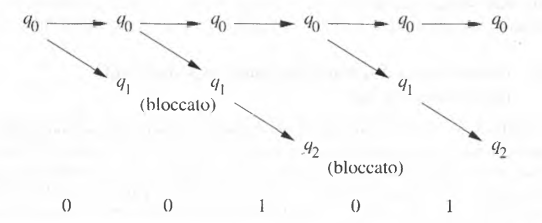
\includegraphics[scale=0.7]{img/nfa.png}
\end{center}
ovvero si parte dallo stato inziale, quando viene letto 0 si passa a $q_0$ e $q_1$, poi viene letto il secondo 0 quindi $q_0$ va nuovamente verso $q_0$ e $q_1$ mentre il primo $q_1$ muore non avendo transizioni su 0. Arriva poi l'1 quindi $q_0$ va solon verso $q_0$ e $q_1$ verso $q_2$ e sarebbe accettante ma l'input non è finito. Ora arriva 0 e $q_2$ si blocca mentre $q_0$ va sia in $q_0$ che in $q_1$. Arriva infine un 1 che manda $q_0$ in $q_0$ e $q_1$ in $q_2$ che è accettante e non avendo altri input si è dimostrata l'appartenenza della stringa al linguaggio
\end{esempio}
definisco quindi un NFA come una quintupla:
$$A=(Q,\Sigma,\delta,q_0,F)$$
con, a differenza dei DFA:
$$\delta:Q\times F\to 2^Q$$
Possiamo ora definire \^{$\delta$}, delta cappuccio che prende in ingresso uno stato e l'intera stringa $w$. Definisco ricorsivamente:
\begin{itemize}
\item \textbf{caso base:} se $|w|=0$ ovvero se $W=\varepsilon$ si ha:
$$\hat{\delta}(q,\varepsilon)=\{q\}$$
\item \textbf{caso passo:} se $|w|>0$, allora $W=xa$, $a\in\Sigma$ e $x\in\Sigma^*$. Posto $\hat{\delta}(q,x)=\{p_1,...,p_k\}$ si ha:
$$\hat{\delta}(q,w)=\cup \delta(p_i,a)$$
\end{itemize}
%aggiungere esempio
Per il lingauggio $L$ accettato dall'automa si ha:
$$L(A)=\{w\in \Sigma^*|\, \hat{\delta}(q_0,q)\cap F\neq \emptyset\}$$
\begin{esempio}
Automa per $L=\{x010y|\,x,y\in\{0,1\}^*\}$ ovvero tutte le stringhe con dentro la sequenza $010$:
\begin{center}
\begin{tikzpicture}[shorten >=1pt,node distance=2cm,on grid,auto] 
\node[state, initial] (q_0) {$q_{0}$};
	\node[state] (q_1) [right=of q_0] {$q_{1}$};
	\node[state] (q_2) [right=of q_1] {$q_{2}$};
	\node[state, accepting] (q_3) [right=of q_2] {$q_{3}$};
	\path[->]
	(q_0) edge  node {0} (q_1)
	      edge [loop above] node {0,1} ()
	(q_1) edge  node {1} (q_2)
	(q_2) edge  node {0} (q_3)
	(q_3)     edge [loop above] node {0,1} ();
\end{tikzpicture}
\end{center}
\end{esempio}
Troviamo ora un algoritmo che trasformi un NFA in un DFA.\\
Dall'ultimo esempio ricavo:
\begin{center}
\begin{tabular}{c|c|c}
& 0 & 1\\
\hline
$\emptyset$ & $\emptyset$ & $\emptyset$ \\
\hline
$\to \,\{q_0\}$ & $\{q_0,q_1\}$ & $\{q_0\}$\\
\hline
$\,\{q_1\}$ & $\emptyset$ & $\{q_2\}$\\
\hline
$*\,\{q_2\}$ & $\emptyset$ & $\emptyset$\\
\hline
$\{q_0,q_1\}$ & $\{q_0,q_1\}$ & $\{q_0,q_2\}$\\
\hline
$*\,\{q_0,q_2\}$ & $\{q_0,q_1\}$ & $\{q_0\}$\\
\hline
$*\,\{q_1, q_2\}$ & $\emptyset$ & $\{q_2\}$\\
\hline
$*\,\{q_0,q_1,q_2\}$ & $\{q_0,q_1\}$ & $\{q_0,q_2\}$
\end{tabular}
\end{center}
ovvero:
\begin{center}
\begin{tikzpicture}[shorten >=1pt,node distance=4cm,on grid,auto] 
\node[state, initial] (q_0) {$\{q_{0}\}$};
	\node[state] (q_1) [right=of q_0] {$\{q_{0}, q_1\}$};
	\node[state] (q_2) [right=of q_1] {$\{q_0,q_{2}\}$};
	\path[->]
	(q_0) edge  node {0} (q_1)
	      edge [loop above] node {1} ()
	(q_1) edge  node {1} (q_2)
	      edge [loop above] node {0} ()
	(q_2) edge [bend left =25]  node {0} (q_1)
	      edge [bend left =45] node  {1} (q_0);
\end{tikzpicture}
\end{center}
che è il DFA che si era anche prima ottenuto. Si hanno però dei sottoinsiemi mai raggiungibili. Si ha quindi:
\begin{center}
\begin{tabular}{c|c|c}
& 0 & 1\\
\hline
$\to\,\{q_0\}$ & $\{q_0,q_1\}$ & $\{q_0\}$ \\
\hline
$\{q_0,q_1\}$ & $\{q_0,q_1\}$ & $\{q_0,q_2\}$\\
\hline
$\,\{q_0, q_2\}$ & $\{q_0,q_1\}$ & $\{q_0\}$
\end{tabular}
\end{center}
e definendo $\{q_0\}=a, \, \{q_0,q_1\}=b\,\,\, e\,\,\, \{q_0,q_2\}=c$ si avrà:
\begin{center}
\begin{tikzpicture}[shorten >=1pt,node distance=2cm,on grid,auto] 
	\node[state, initial] (q_0) {$a$};
	\node[state] (q_1) [right=of q_0] {$b$};
	\node[state, accepting] (q_2) [right=of q_1] {$c$};
	\path[->]
	(q_0) edge  node {0} (q_1)
	      edge [loop above] node {1} ()
	(q_1) edge  node {1} (q_2)
	      edge [loop above] node {0} ()
	(q_2) edge  [bend left =25] node {0} (q_1)
	      edge [bend left = 50] node {1} (q_0);
\end{tikzpicture}
\end{center}
Definiamo questo algoritmo che avrà:
\begin{itemize}
\item come input un NFA $N=(Q_n,\Sigma,\delta_N,q_0,F_N)$
\item come output un DFA $D=(Q_D,\Sigma,\delta_D,\{q_0\},F_D)$ tale che $L(D)=L(N)$
\end{itemize}
con:
\begin{itemize}
\item $Q_D=2^{Q_N}$ (quindi se $Q_N=n$ si ha $|Q_D|=2^n$)
\item $F_D=\{S\subseteq Q_n|\, S\cap F_N\neq \emptyset\}$
\item $\forall S\subseteq Q_N$ e $ \forall a \in\Sigma$:
$$\delta_D(S,a)=\cup \delta_n(p,a)$$
per esempio:
$$\delta_D(\{q_0,q_1,q_2\},0)=\delta_N(q_0,0)\cup \delta_N(q_1,0) \cup\delta_N(q_2,0) $$ 
\end{itemize}
Si definisce l'$\varepsilon-NFA$, l'automa astati finiti non deterministici con $\varepsilon$ transizioni. Con la transizione $\varepsilon$ posso saltare i nodi, ovvero avanza senza aggiungere caratteri
\begin{esempio}
Si ha $ER=a^*b^*c^*$, che genera:
$$L=\{a^nb^mc^k|\,n,m,k\geq 0\}$$
si ha:
\begin{center}
\begin{tikzpicture}[shorten >=1pt,node distance=2cm,on grid,auto] 
	\node[state, initial] (q_0) {$q_0$};
	\node[state] (q_1) [right=of q_0] {$q_1$};
	\node[state, accepting] (q_2) [right=of q_1] {$q_2$};
	\path[->]
	(q_0) edge  node {$\varepsilon$} (q_1)
	      edge [loop above] node {a} ()
	(q_1) edge  node {$\varepsilon$} (q_2)
	      edge [loop above] node {b} ()
	(q_2) edge  [loop above] node {c} ();
\end{tikzpicture}
\end{center}
ovvero con $\varepsilon$ posso per esempio generare quante $a$ voglio da $q_0$ e passare a $q_2$, uscendo senza generare altro
\end{esempio}
Si definisce la funzione $E\,CLOSE:Q\to 2^Q$, con $E\,CLOSE(q)$ insieme degli stati raggiungibili da $q$ tramite $\varepsilon-mosse$. Nell'esempio precedente si avrebbe:
$$E\,CLOSE(q_0)=\{q_0,q_1,q_2\}$$
$$E\,CLOSE(q_1)=\{q_1,q_2\}$$
$$E\,CLOSE(q_2)=\{q_2\}$$
si ha inoltre che:
\begin{itemize}
\item $E\,CLOSE 2^Q\to 2^Q\,\,\, P\subseteq Q$
\item $E\,CLOSE(P)=\cup E\,CLOSE(p)$
\item $E\,CLOSE(\emptyset)=\emptyset$
\end{itemize}
mettendo in tabella l'esempio precedente si ha:
\begin{center}
\begin{tabular}{c|c|c|c}
& a & b & c\\
\hline
$*\to\,\{q_0,q_1,q_2\}$ & $\{q_0,q_1,q_2\}$ & $\{q_1,q_2\}$ & $\{q_2\}$\\
\hline
$*\{q_1,q_2\}$ & $\emptyset$ & $\{q_1,q_2\}$ & $\{q_2\}$\\
\hline
$*\{q_2\}$ & $\emptyset$ & $\emptyset$ & $\{q_2\}$\\
\hline
$\emptyset$ & $\emptyset$ & $\emptyset$ & $\emptyset$ 
\end{tabular}
\end{center}
riscrivendo:
\begin{itemize}
\item $a=\{q_0,q_1,q_2\}$
\item $b=\{q_1,q_2\}$
\item $c=\{q_2\}$
\item $d=\emptyset$
\end{itemize}
ovvero:
$$\delta_D(\{q_0,q_1,q_2\},a)=E\,CLOSE(\delta_N(q_0,a)\cup \delta_N(q_1,a)\cup \delta_N(q_2,a))$$
$$=E\,CLOSE(\{q_0\} \cup \emptyset\cup \emptyset)=E\,CLOSE(\{q_0\})$$
$$=E\,CLOSE	(q_0)=\{q_0,q_1,q_2\}$$
e
$$\delta_D(\{q_0,q_1,q_2\},B)=E\,CLOSE(\delta_N(q_0,b)\cup \delta_N(q_1,b)\cup \delta_N(q_2,b))$$
$$=E\,CLOSE(\emptyset \cup \{q_1\}\cup \emptyset)=E\,CLOSE(\{q_1\})$$
$$=E\,CLOSE	(q_1)=\{q_1,q_2\}$$
e
$$\delta_D(\{q_0,q_1,q_2\},c)=E\,CLOSE(\delta_N(q_0,c)\cup \delta_N(q_1,c)\cup \delta_N(q_2,c))$$
$$=E\,CLOSE(\emptyset \cup \emptyset\cup \{q_2\})=E\,CLOSE(\{q_1\})$$
$$=E\,CLOSE	(q_2)=\{q_2\}$$
\newpage
si ottiene quindi il seguente NFA:
\begin{center}
\begin{tikzpicture}[shorten >=1pt,node distance=3cm,on grid,auto] 
	\node[state, initial, accepting] (q_0) {$A$};
	\node[state, accepting] (q_1) [right=of q_0] {$B$};
	\node[state, accepting] (q_2) [below=of q_0] {$C$};
	\node[state] (q_3) [right=of q_2] {$D$};
	\path[->]
	(q_0) edge  node {b} (q_1)
	      edge  node {c} (q_2)
	      edge [loop above] node {a} ()
	(q_1) edge  node {c} (q_2)
	      edge  node {a} (q_3)
	      edge [loop above] node {b} ()
	(q_2) edge  node {a,b} (q_3)
	      edge [loop below] node {c} ()
	(q_3) edge [loop below] node {a,b,c} ();
\end{tikzpicture}
\end{center}
che diventa il seguente DFA:
\begin{center}
\begin{tikzpicture}[shorten >=1pt,node distance=3cm,on grid,auto] 
	\node[state, initial, accepting] (q_0) {$\{q_0,q_1,q_2\}$};
	\node[state, accepting] (q_1) [right=of q_0] {$\{q_1,q_2\}$};
	\node[state, accepting] (q_2) [below=of q_0] {$\{q_2\}$};
	\node[state] (q_3) [right=of q_2] {$q_E$};
	\path[->]
	(q_0) edge  node {b} (q_1)
	      edge  node {c} (q_2)
	      edge [loop above] node {a} ()
	(q_1) edge  node {c} (q_2)
	      edge  node {a} (q_3)
	      edge [loop above] node {b} ()
	(q_2) edge  node {a,b} (q_3)
	      edge [loop below] node {c} ();
\end{tikzpicture}
\end{center}
\newpage
\subsubsection{esercizi}
\begin{esempio}
automa DFA per $w=x010y,\,x,y\in\{0,1\}^*$ :\\
la stringa più corta è 010
\begin{center}
\begin{tikzpicture}[shorten >=1pt,node distance=2cm,on grid,auto] 
\node[state, initial] (q_0) {$q_{0}$};
	\node[state] (q_1) [right=of q_0] {$q_{1}$};
	\node[state] (q_2) [right=of q_1] {$q_{2}$};
	\node[state, accepting] (q_3) [right=of q_2] {$q_{3}$};
	\path[->]
	(q_0) edge  node {0} (q_1)
	      edge [loop above] node {1} ()
	(q_1) edge  node {1} (q_2)
	      edge [loop above] node {0} ()
	(q_2) edge  node {0} (q_3)
	      edge  [bend left = 45] node {1}(q_0)
	(q_3) edge [loop above] node {0,1} ();
\end{tikzpicture}
\end{center}
\end{esempio}
\begin{esempio}
automa DFA per $a^{2k+1}b^{2h},\, h,k\geq 0$ :\\
concatenazione di a dispari e b pari:
\begin{center}
\begin{tikzpicture}[shorten >=1pt,node distance=2cm,on grid,auto] 
	\node[state, initial] (q_0) {$q_{0}$};
	\node[state, accepting] (q_1) [right=of q_0] {$q_{1}$};
	\node[state] (q_3) [right=of q_1] {$q_{3}$};
	\node[state] (q_2) [below= of q_1] {$q_{2}$};
	\node[state, accepting] (q_4) [right = of q_2] {$q_4$};
	\node[state] (q_5) [right=of q_4] {$q_E$};
	\path[->]
	(q_0) edge  node [bend left = 25] {a} (q_1)
	(q_1) edge [bend left = 25] node {a} (q_2)
	      edge node [bend left= 25] {b} (q_3)
	(q_2) edge [bend left = 25] node [left] {a} (q_1)
	(q_3) edge [bend right = 25] node [left] {b} (q_4)
	(q_4) edge [bend right = 25] node [right] {b} (q_3)
	(q_2) edge  [bend right = 55] node [below] {b} (q_5)
	(q_3) edge  [bend left = 25] node {a} (q_5)
	(q_4) edge  [bend right = 25] node [below] {a} (q_5)
	(q_5) edge [loop right] node {a,b} ();
\end{tikzpicture}
\end{center}
\end{esempio}
\begin{esempio}
cerco DFA per stringhe inizianti con a e finenti con b, con occorrenze di b singole o a coppie, nessuna regola per c.\\
per esempio $abbcb$ è nel linguaggio
\begin{center}
\begin{tikzpicture}[shorten >=1pt,node distance=2cm,on grid,auto] 
	\node[state, initial] (q_0) {$q_{0}$};
	\node[state] (q_1) [right=of q_0] {$q_{1}$};
	\node[state, accepting] (q_2) [right=of q_1] {$q_{2}$};
	\node[state, accepting] (q_3) [right= of q_3] {$q_{3}$};
	\node[state] (q_5) [below=of q_0] {$q_E$};
	\path[->]
	(q_0) edge  node [bend left = 25] {a} (q_1)
		  edge  node [bend left = 25] {b,c} (q_5)
	(q_1) edge  node {b} (q_2)
	      edge [loop] node {a,c} ()
	(q_2) edge [bend left = 25] node {a,c} (q_1)
	      edge  node  {b} (q_3)
	(q_3) edge [bend left = 65] node [below] {b} (q_5)
	      edge [bend left = 55] node {a,c} (q_1)
	(q_5) edge [loop left] node {a,b,c} ();
\end{tikzpicture}
\end{center}
\end{esempio}
\newpage
\begin{esempio}
cerco DFA per  stringhe di bit non contegano 000
\begin{center}
\begin{tikzpicture}[shorten >=1pt,node distance=2cm,on grid,auto] 
    \node[state, initial, accepting] (q_0) {$q_0$};
    \node[state, accepting] (q_1) [right=of q_0]{$q_1$};
    \node[state, accepting] (q_2) [right=of q_1]{$q_2$};
    \node[state] (q_e) [right=of q_2]{$q_E$};
    \path[->]
    (q_0) edge  [bend left=25] node {0} (q_1)
          edge [loop] node {1} ()
    (q_1) edge node {0} (q_2)
          edge [bend left=25] node {1} (q_0)
    (q_2) edge node {0} (q_e)
          edge  [bend left=55] node{1} (q_0)
    (q_e) edge [loop ] node {0,1} ();
\end{tikzpicture}
\end{center}
\end{esempio}
\begin{esempio}
cerco DFA per  stringhe di bit non contegano 000 almeno una volta
\begin{center}
\begin{tikzpicture}[shorten >=1pt,node distance=2cm,on grid,auto] 
    \node[state, initial] (q_0) {$q_0$};
    \node[state] (q_1) [right=of q_0]{$q_1$};
    \node[state] (q_2) [right=of q_1]{$q_2$};
    \node[state, accepting] (q_e) [right=of q_2]{$q_E$};
    \path[->]
    (q_0) edge  [bend left=25] node {0} (q_1)
          edge [loop] node {1} ()
    (q_1) edge node {0} (q_2)
          edge [bend left=25] node {1} (q_0)
    (q_2) edge node {0} (q_e)
          edge  [bend left=55] node{1} (q_0)
    (q_e) edge [loop ] node {0,1} ();
\end{tikzpicture}
\end{center}
\end{esempio}
\begin{esempio}
cerco DFA per  stringhe di bit che contengono 000 solo una volta
\begin{center}
\begin{tikzpicture}[shorten >=1pt,node distance=2cm,on grid,auto] 
    \node[state, initial] (q_0) {$q_0$};
    \node[state] (q_1) [right=of q_0]{$q_1$};
    \node[state] (q_2) [right=of q_1]{$q_2$};
    \node[state, accepting] (q_3) [right=of q_2]{$q_3$};
    \node[state,accepting] (q_4) [below=of q_3] {$q_3$};
    \node[state] (q_5) [below=of q_4]{$q_5$};
    \node[state] (q_6) [below=of q_5]{$q_6$};
    \node[state] (q_e) [right=of q_3]{$q_E$};
    \path[->]
    (q_0) edge  [bend left=25] node {0} (q_1)
          edge [loop] node {1} ()
    (q_1) edge node {0} (q_2)
          edge [bend left=25] node {1} (q_0)
    (q_2) edge node {0} (q_3)
          edge  [bend left=45] node{1} (q_0)
    (q_3) edge node {0} (q_e)
          edge node {1} (q_4)
    (q_4) edge [bend left=25] node {0} (q_5)
    	  edge [loop right] node {1} ()
    (q_5) edge [bend left=25] node {1} (q_4)
          edge node {0} (q_6)
    (q_6) edge [bend right=25] node {0} (q_e)
          edge [bend left=55] node {0} (q_4)
    (q_e) edge [loop ] node {0,1} ();
\end{tikzpicture}
\end{center}
\end{esempio}
\newpage
\begin{esempio}
Trasformare il seguente NFA in un DFA:
\begin{center}
\begin{tikzpicture}[shorten >=1pt,node distance=3cm,on grid,auto] 
	\node[state, initial, accepting] (q_0) {$q_0$};
	\node[state, accepting] (q_1) [above right=of q_0] {$q_1$};
	\node[state] (q_2) [below right =of q_0] {$q_2$};
	\node[state] (q_3) [below right=of q_1] {$q_3$};
	\path[->]
	(q_0) edge  [bend left=25] node {a} (q_1)
	      edge  [bend right=25] node [below] {b} (q_2)
	(q_1) edge  [bend left=25] node {a} (q_2)
	      edge [loop ] node {a} ()
	(q_2) edge  [bend left=25] node {b} (q_1)
	      edge  [bend right=15] node [below] {b} (q_3)
	(q_3) edge   node [above] {a} (q_1)
	      edge  [bend right=15] node [above] {a} (q_2);
\end{tikzpicture}
\end{center}
abbiamo quindi:
$$\delta_D(\{q_0\},a)=\delta_N(q_0,a)=\{q_1,q_2\}$$
$$\delta_D(\{q_0\},b)=\delta_N(q_1,b)=\emptyset$$
$$\delta_D(\{q_1,q_2\},a)=\delta_N(q_1,a)\cup \delta_N(q_2,a)=\{q_1,q_2\}cup \emptyset=\{q_1,q_2\}$$
$$\delta_D(\{q_1,q_2\},b)=\delta_N(q_1,b)\cup \delta_N(q_2,b)=\emptyset\cup \{q_1,q_3\}=\{q_1,q_3\}$$
$$...$$
ottengo quindi:
\begin{center}
\begin{tabular}{c|c|c}
DFA & a & b \\
\hline
$*\to\,\{q_0\}$ & $\{q_1,q_2\}$ & $\emptyset$ \\
\hline
$*\{q_1,q_2\}$ & $\{q_1,q_2\}$ & $\{q_1,q_3\}$ \\
\hline
$\emptyset$ & $\emptyset$ & $\emptyset$ \\
\hline
$*\{q_1,q_3\}$ & $\{q_1,q_2\}$ & $\emptyset$ 
\end{tabular}
\end{center}
Posso ora rinominare:
\begin{itemize}
\item $A=\{q_0\}$
\item $B=\{q_1,q_2\}$
\item $C=\emptyset$
\item $D=\{q_1,q_3\}$
\end{itemize}
\newpage
ottengo quindi il seguente DFA:
\begin{center}
\begin{tikzpicture}[shorten >=1pt,node distance=3cm,on grid,auto] 
	\node[state, initial, accepting] (q_0) {$A$};
	\node[state, accepting] (q_1) [right=of q_0] {$B$};
	\node[state] (q_2) [below=of q_0] {$C$};
	\node[state,accepting] (q_3) [right=of q_2] {$D$};
	\path[->]
	(q_0) edge  node {a} (q_1)
	      edge  node {b} (q_2)
	(q_1) edge  [bend left=25] node {b} (q_3)
	      edge  [loop] node {a} ()
	(q_2) edge  [loop below] node {a,b} ()
	(q_3) edge  [bend left=25] node {a} (q_1)
	      edge  node  {a} (q_2);
\end{tikzpicture}
\end{center}
\end{esempio}
\begin{esempio}
Trasformare il seguente $\varepsilon$-NFA in un DFA:
\begin{center}
\begin{tikzpicture}[shorten >=1pt,node distance=3cm,on grid,auto] 
	\node[state, initial] (q_0) {$p$};
	\node[state] (q_1) [right=of q_0] {$q$};
	\node[state, accepting] (q_2) [below right =of q_0] {$r$};
	\path[->]
	(q_0) edge  [bend left=25] node [left] {c} (q_2)
	      edge  [bend right=25] node {b} (q_1)
	      edge [loop ] node {a} ()
	(q_1) edge  [bend right=25] node {$\varepsilon$} (q_0)
	      edge  [bend right=25] node [left] {b} (q_2)
	      edge  [loop ] node {a} ()
	(q_2) edge  [bend left=25] node {c} (q_0)
	      edge  [bend right=25] node [right] {$\varepsilon$} (q_1)
	      edge  [loop below] node {a} ();
\end{tikzpicture}
\end{center}
vediamo le ECLOSE:
$$ECLOSE(p)=\{p\}$$
$$ECLOSE(q)=\{p,q\}$$
$$ECLOSE(r)=\{p,q,r\}$$
si ottiene quindi:
\begin{center}
\begin{tabular}{c|c|c|c}
 & a & b & c\\
\hline
$to\,\{p\}$ & $\{p\}$ & $\{p,q\}$ & $\{p,q,r\}$\\
\hline
$\{p,q\}$ & $\{p,q\}$ & $\{p,q,r\}$ & $\{p,q,r\}$\\
\hline
$*\{p,q,r\}$ & $\{p,q,r\}$ & $\{p,q,r\}$ & $\{p,q,r\}$
\end{tabular}
\end{center}
infatti, per esempio:
$$\delta_D(\{p\}, a)= ECLOSE (\delta_(p,a))=ECLOSE (\{p\})=ECLOSE (p)=\{p\}$$
$$\delta_D(\{p,q\}, a)= ECLOSE (\delta_N(p,a)\cup \delta_N(q,a))=$$
$$ECLOSE (\{p\}\cup \{q\})=ECLOSE(P)\cup ECLOSE(q)=\{p\}\cup\{p,q\}=\{p,q\}$$
$$...$$
si hanno quindi le seguenti rinominazioni:
\begin{itemize}
\item $A=\{p\}$
\item $b=\{p,q\}$
\item $C=\{p,q,r\}$
\end{itemize}
ovvero:
\begin{center}
\begin{tikzpicture}[shorten >=1pt,node distance=3cm,on grid,auto] 
	\node[state, initial] (q_0) {$A$};
	\node[state] (q_1) [right=of q_0] {$B$};
	\node[state, accepting] (q_2) [below=of q_0] {$C$};
	\path[->]
	(q_0) edge  node {b} (q_1)
	      edge  node {c} (q_2)
	      edge  [loop] node {a} ()
	(q_1) edge  node {b,c} (q_2)
	      edge  [loop] node {a} ()
	(q_2) edge  [loop below] node {a,b,c} ();
\end{tikzpicture}
\end{center}
\end{esempio}